% !TEX root =../main.tex

\chapter{Konzeptionierung}

In diesem Kapitel wird dargestellt, wie ein Teil der Implementierung durchgeführt werden können. Angenommen, der Nutzer A will ein Computer in einem Webshop kaufen. Er besitzt nicht die Kenntnisse im Bereich von Hardware und Software um dies eigenständig zu tun. Eine Konfiguration vor Parametern fällt ihm Schwer. Er braucht die Hilfe von anderen Leuten.


\section{Prozessmodell zur Beschreibung des Kaufprozesses}

Für eine Konzeptionierung müssen die Prozesse analysiert und auf ihren Ablauf überprüft werden. Grundlage für eine solche Analyse ist die strukturierte Darstellung des Einkaufsprozesses. Die Prozessmodellierungssprache „Business Process Model and Notation“ (BPMN) soll dabei die Zusammenarbeit zwischen Nutzer, Verkäufer und dem System erleichtern. Ziel dieser Studie ist es, den Handelsablauf und die Informationsflüsse zwischen unterschiedlichen Akteuren zu zeigen und mittels BMPN 2.0 zu visualisieren.


\subsection{Prozessmodellierung mit BPMN}

BPMN (Business Process Model and Notation) ist eine graphenbasierte Notationssprache, die von der Object Management Group erstmals im Jahre 2004 veröffentlicht wurde und seit Anfang des Jahres 2011 in Version 2.0 vorliegt. \parencite{bpmn} Unternehmen und Organisationen verwenden BPMN, um ihre Geschäftsprozesse für das Prozessmanagement zu dokumentieren und zu konfigurieren.


\subsection{Einkaufsprozess}

Im Anschluss an die Erhebung wurde der Prozess des Einkaufens in einem BPMN-Modell umgesetzt. Die Wahl einer Prozessmodellierungssprache und -technik fiel auf BPMN, da diese den Anspruch hat, sowohl von inhaltlichen Fachleuten (Prozesskenner) als auch technischen Experten (Entwickler) gelesen und verstanden zu werden. \parencite{allweyer}

Abbildung \vref{fig:bpmn-ablauf-kaufen} zeigt den modellierten Einkaufsprozess.

\begin{figure}[htbp]
	\centering
	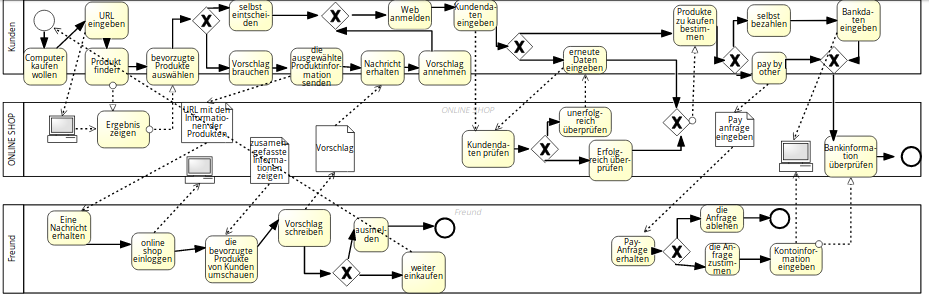
\includegraphics[width=1\textwidth]{bilder/bpmn-ablauf-kaufen.png}
	\caption{Ablauf des Kaufprozess}
	\label{fig:bpmn-ablauf-kaufen}
\end{figure}


\section{Anwendungsfälle}

In den folgenden Abschnitten werden die laut der Autorin wichtigsten Anwendungsfälle definiert und erläutert. Hierbei handelt es sich um die wichtigsten Kernfunktionen des konzipierten Social Commerce Webshops.


\subsection{Freunde einladen}

Um Freunde einzuladen wird durch das System eine URL generiert. Die URL enthält einen einmal gültigen Token an der Sitzung im Webshop teilnehmen zu können. Diese generierte URL wird an einen Freund gesendet.

Wenn ein Freund die Linkinformationen erhält, kann er direkt auf den Link klicken und ohne Anmeldung Beratung geben. Dann kann der Benutzer eine Entscheidung treffen und die Freunde können ausloggen oder weiter einkaufen.

\begin{figure}[htbp]
	\centering
	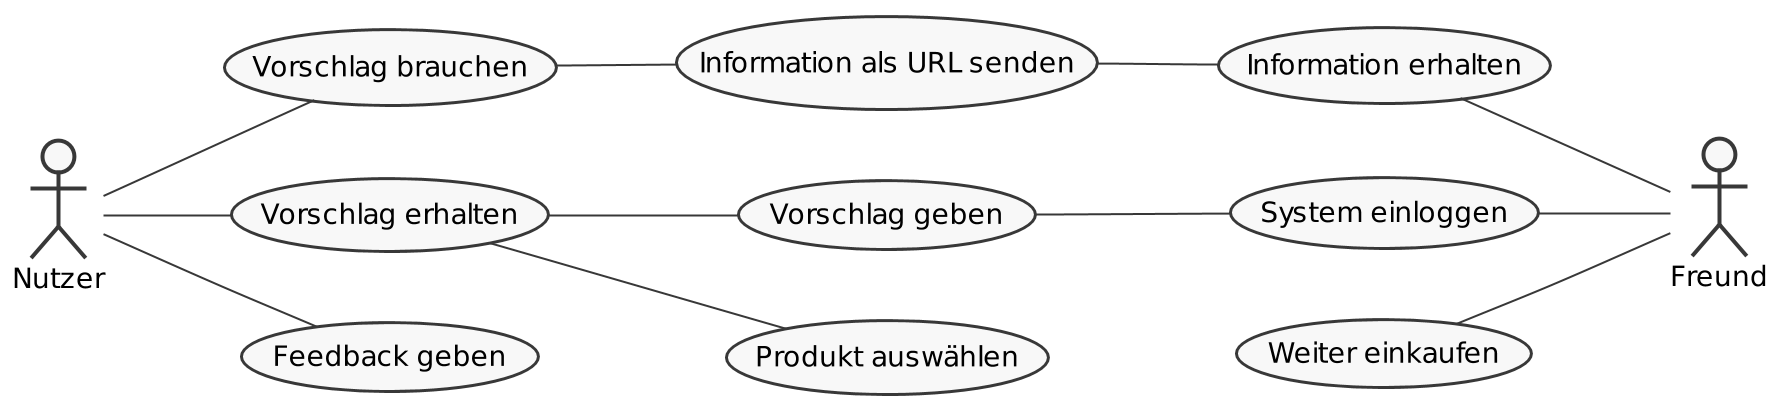
\includegraphics[width=1\textwidth]{uml-diagramme/freunde-einladen.png}
	\caption{Freunde einladen}
	\label{fig:freunde-einladen}
\end{figure}


\subsection{Pay by Others}

Wenn ein Benutzer auf ein Zahlungsproblem stößt, z. B. eine Kreditkarte gesperrt wurde, kann er eine Zahlungsanforderung an einen Freund senden. Freunde beziehen sich hier nicht nur auf Freunde, sondern beziehen sich auch auf andere Bekannte, wie Eltern, Brüder, Schwestern, Freunde, Verwandte und so weiter. Der Freund erhält die Anfrage, überprüft die Bestellung zuerst oder später und entscheidet sich dann für die Annahme oder Ablehnung.

Nachdem die Zahlung abgeschlossen ist, speichert das System automatisch die Zahlungsinformationen und sendet die Zahlungserfolgs- oder Fehlerinformationen an den Benutzer und den Freund.

\begin{figure}[htbp]
	\centering
	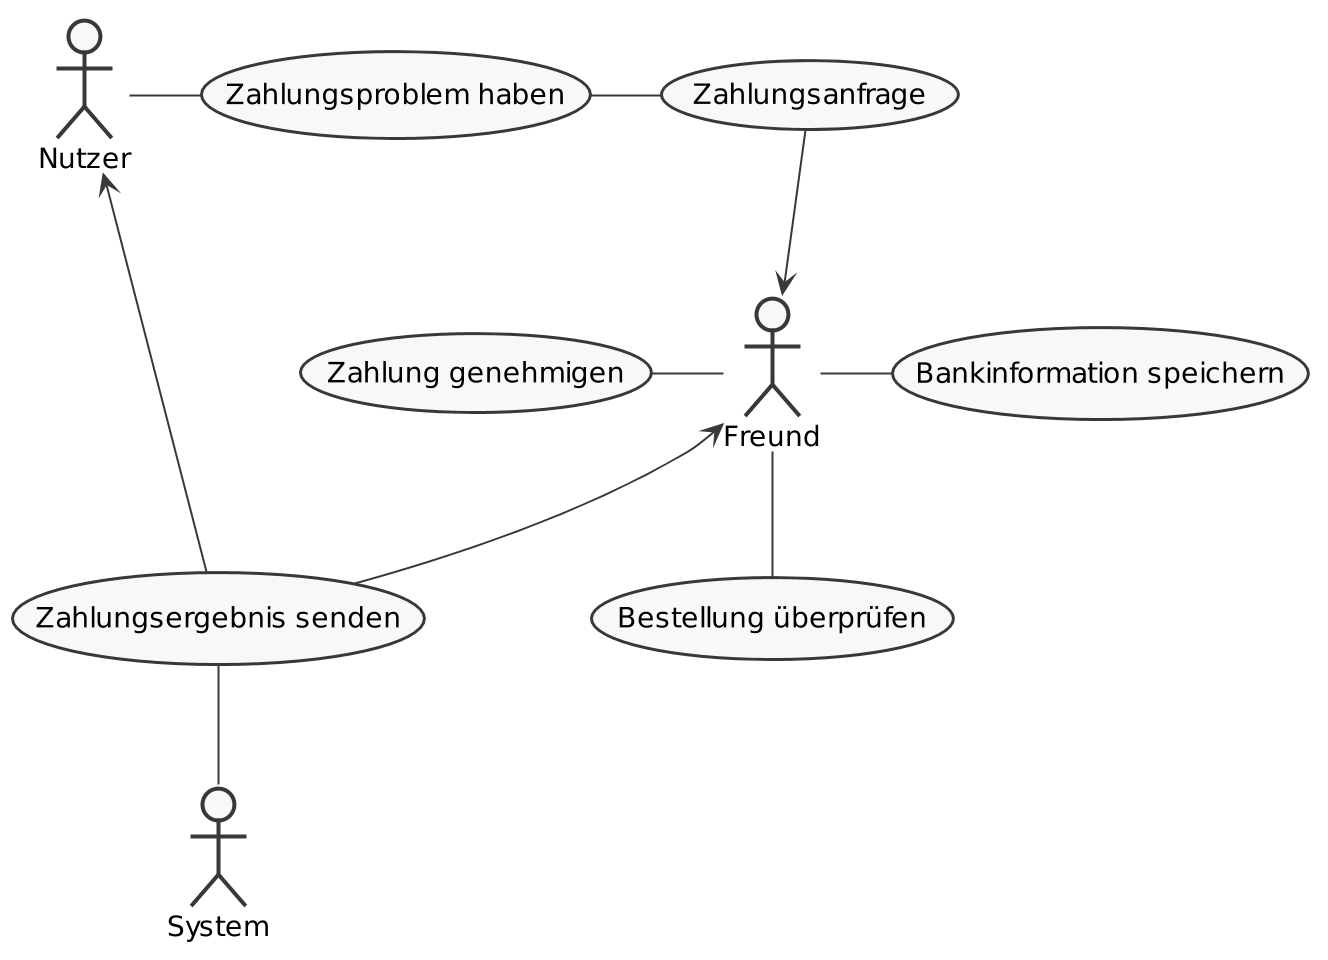
\includegraphics[width=0.8\textwidth]{uml-diagramme/pay-by-others.png}
	\caption{Pay by Others}
	\label{fig:pay-by-others}
\end{figure}


\subsection{Realtime Kommunikation}

Auf dieser Website sind drei Hauptbeteiligte an der Transaktion beteiligt: Nutzer, Freunde und Verkäufer. Das System bietet ein Online-Chat-Tool für die  drei Akteure. Sie  verwenden es, um Produktprobleme zu besprechen, Ratschlägen auszutauschen, Hilfe und Feedback zu geben. Wenn die Nachricht bei der Applikation nicht gesendet wird, beispielsweise wenn ein Akteur offline ist, wird die Nachricht  auf dem Server gespeichert, bis der Teilnehmer wieder online ist.

\begin{figure}[htbp]
	\centering
	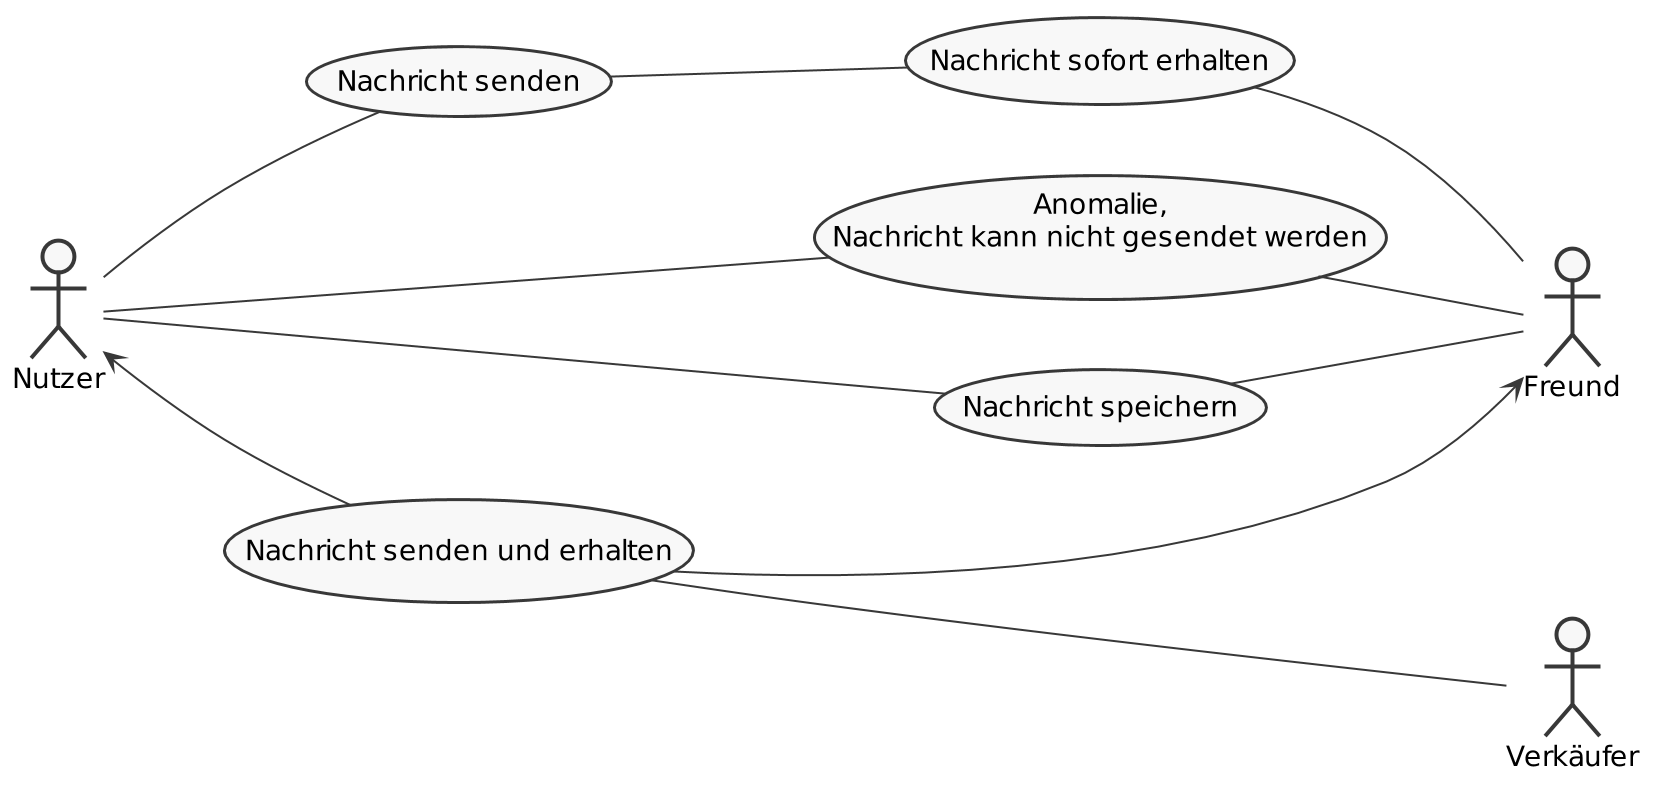
\includegraphics[width=0.8\textwidth]{uml-diagramme/real-time-communication.png}
	\caption{Realtime Kommunikation}
	\label{fig:real-time-communication}
\end{figure}
